%--------------------------------------------------------------------------
% !TEX root = 5Blman.tex
% lenses.tex
% 2013.01.07 changed to 2col format
%--------------------------------------------------------------------------
\chapter{Thin Lenses and Their Images}

\begin{multicols}{2}
%---------------------------------------------------------------------
\section{Purpose}
  The purpose of these laboratory exercises is to give you hands-on experience with thin lenses and the images they form. In this lab, you will also determine the focal length of a lens, determine image distances and magnifications, and verify the thin lens equation.
  
%\begin{wrapfigure}[13]{r}[90pt]{0pt}	
%  \centering
%  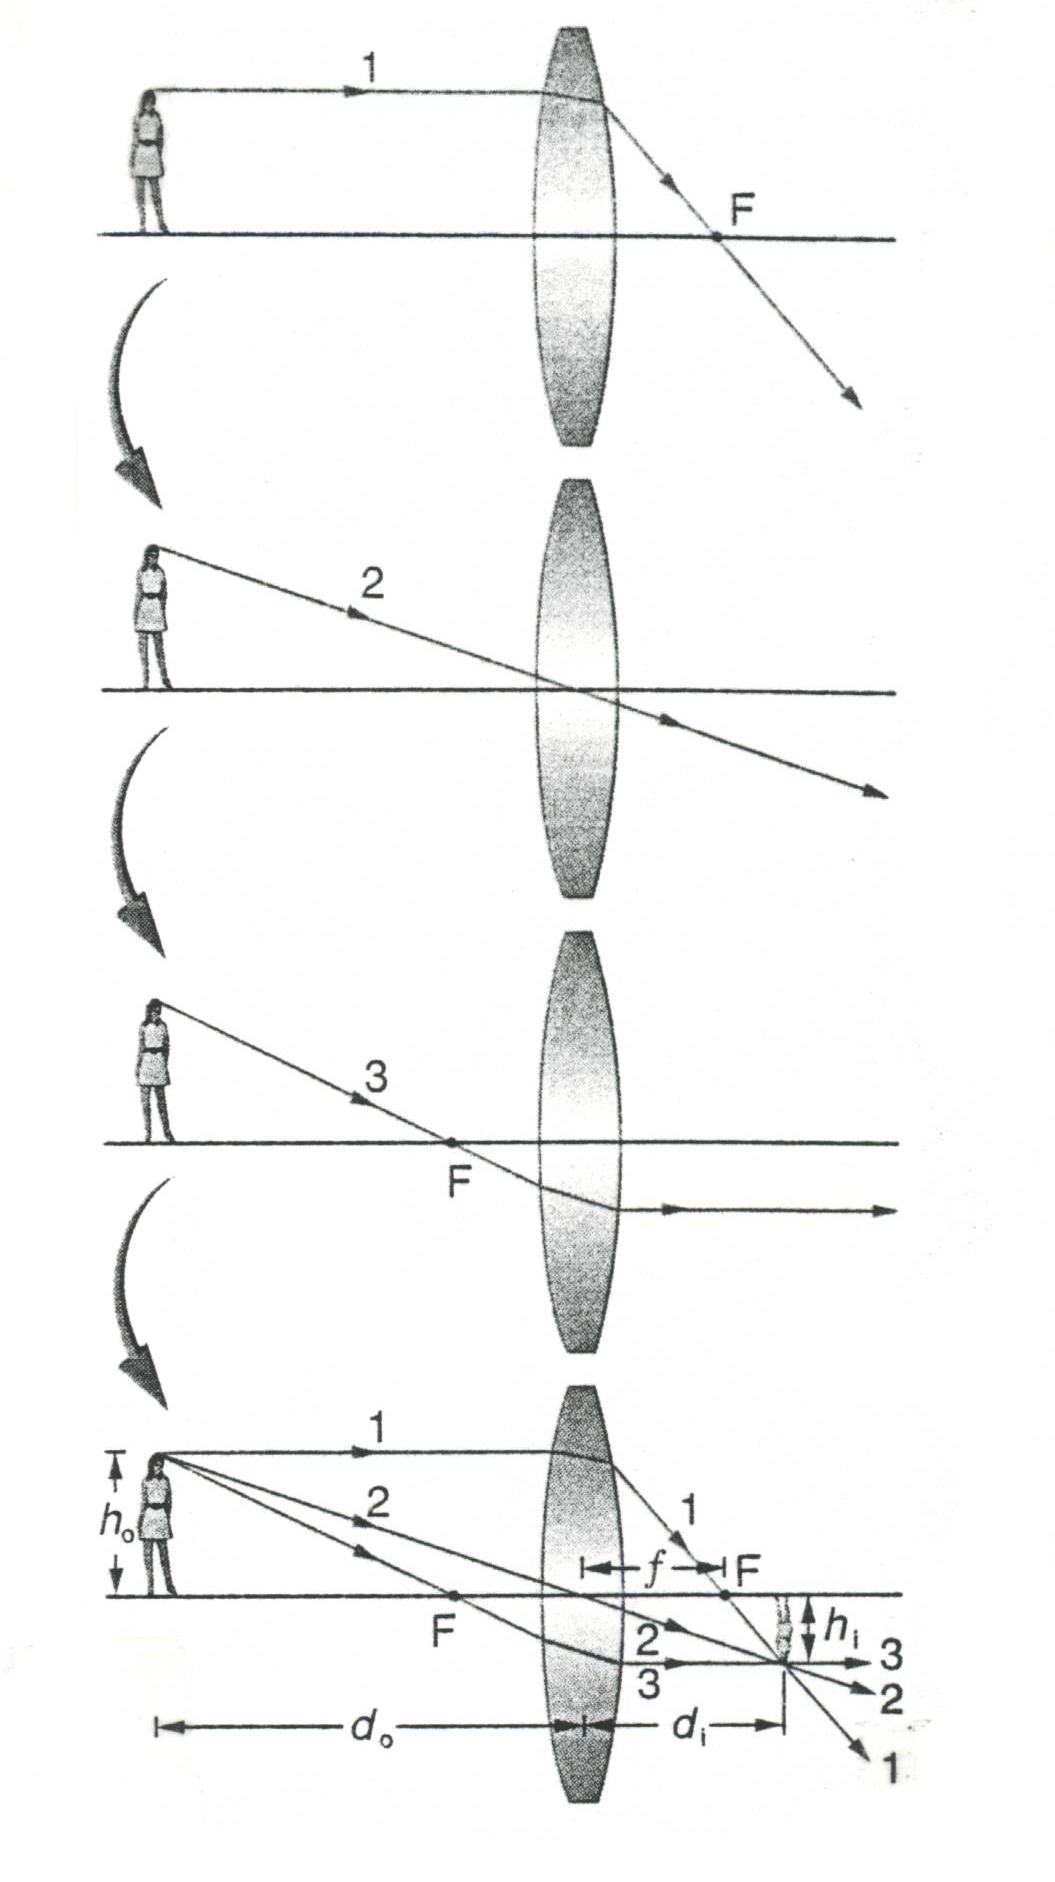
\includegraphics[scale=0.7]{5bgraf/fig_17}
%  \label{f:fig17}
%  \caption{Ray tracing}
%\end{wrapfigure}

%\parpic[r]{\fbox{\Large\scshape Box}}
%\newcommand\FIG{\includegraphics%		 set path on next line
%                 [scale=0.6]{5bgraf/fig_17}}
%                  [width=4cm]{5bgraf/fig_17}}
%                  [width=110pt]{5bgraf/fig_17}}
%\parpic[r]{\FIG}

% may get unpredictable behavior if order is not followed. Option cmds precede \parpic, followed by text. There should be enough text to 'cover' the figure.


%\piccaptiontopside
%\piccaption{Ray tracing} 
%\label{f:fig17}
%\parpic(4cm,6cm)(40mm,110mm)[r]{\FIG}
%\picskip{2}

%---------------------------------------------------------------------
\section{Preparation}
Reread the sections in your text on thin lenses.  Pay particular attention to the technique of ray tracing and the application of the thin lens equations for image formation by lenses.  Become familiar with the three types of images that can be formed by a single thin lens and the conditions under which each type is formed.

\paragraph{Short quiz}
  Be prepared to take a short quiz at the beginning of lab related to the concepts associated with this laboratory exercise.

%---------------------------------------------------------------------
\section{General Information}

%\piccaption{Ray tracing} 
%\label{f:fig17}
%\parpic(0cm,0cm)(40mm,70mm)[r]{\FIG}
%\picskip{2}

The technique of ray tracing is used to find the location and type of image formed by an optical system. In your text you will find several examples of ray tracing that are pertinent to this laboratory exercise. \reffig{f:fig17} shows a step-by-step illustration of ray tracing for a convex lens with an object at a distance greater than the focal length of the lens.  When ray tracing is performed carefully to scale it accurately predicts information about the size and location of images formed by optical instruments.

%\begin{figure}
%	\centering
%	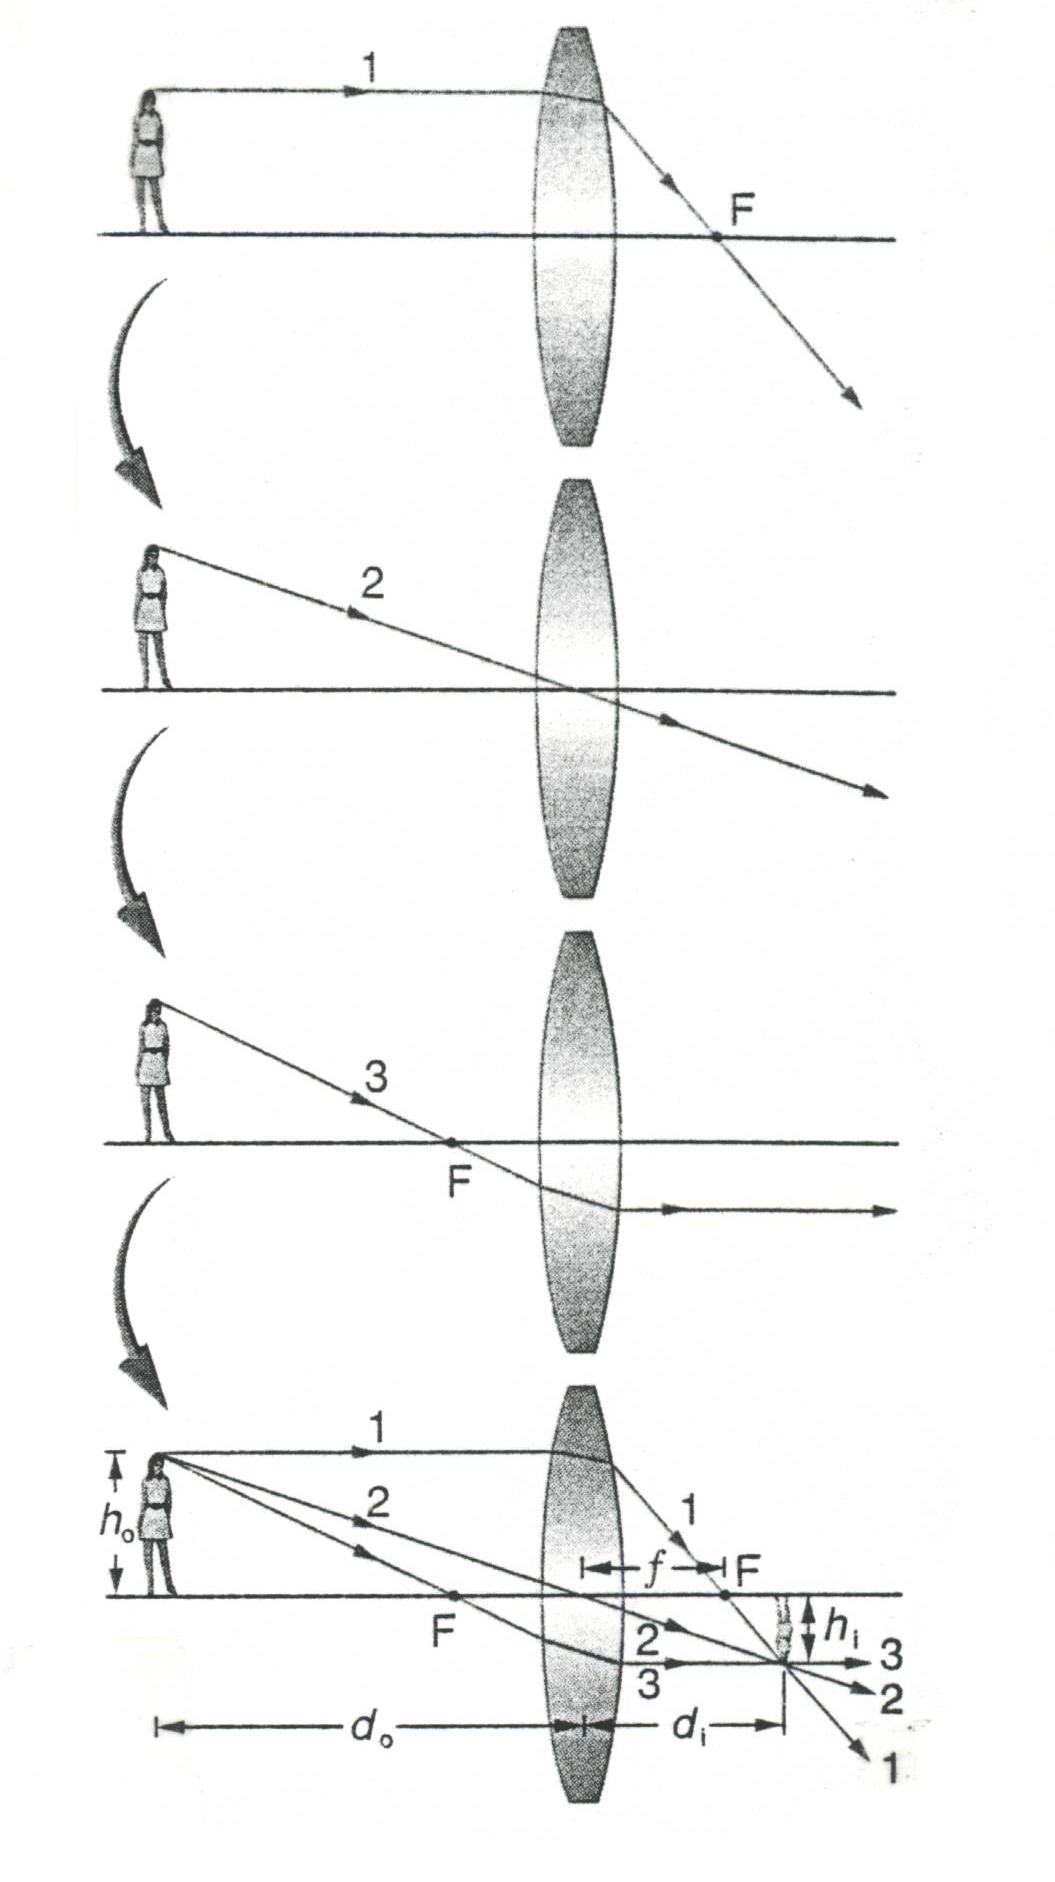
\includegraphics[scale=0.7]{5bgraf/fig_17}
%	\caption{Ray tracing is used to locate the image formed by a lens}
%	\label{f:fig17}
%\end{figure}

\begin{center}
	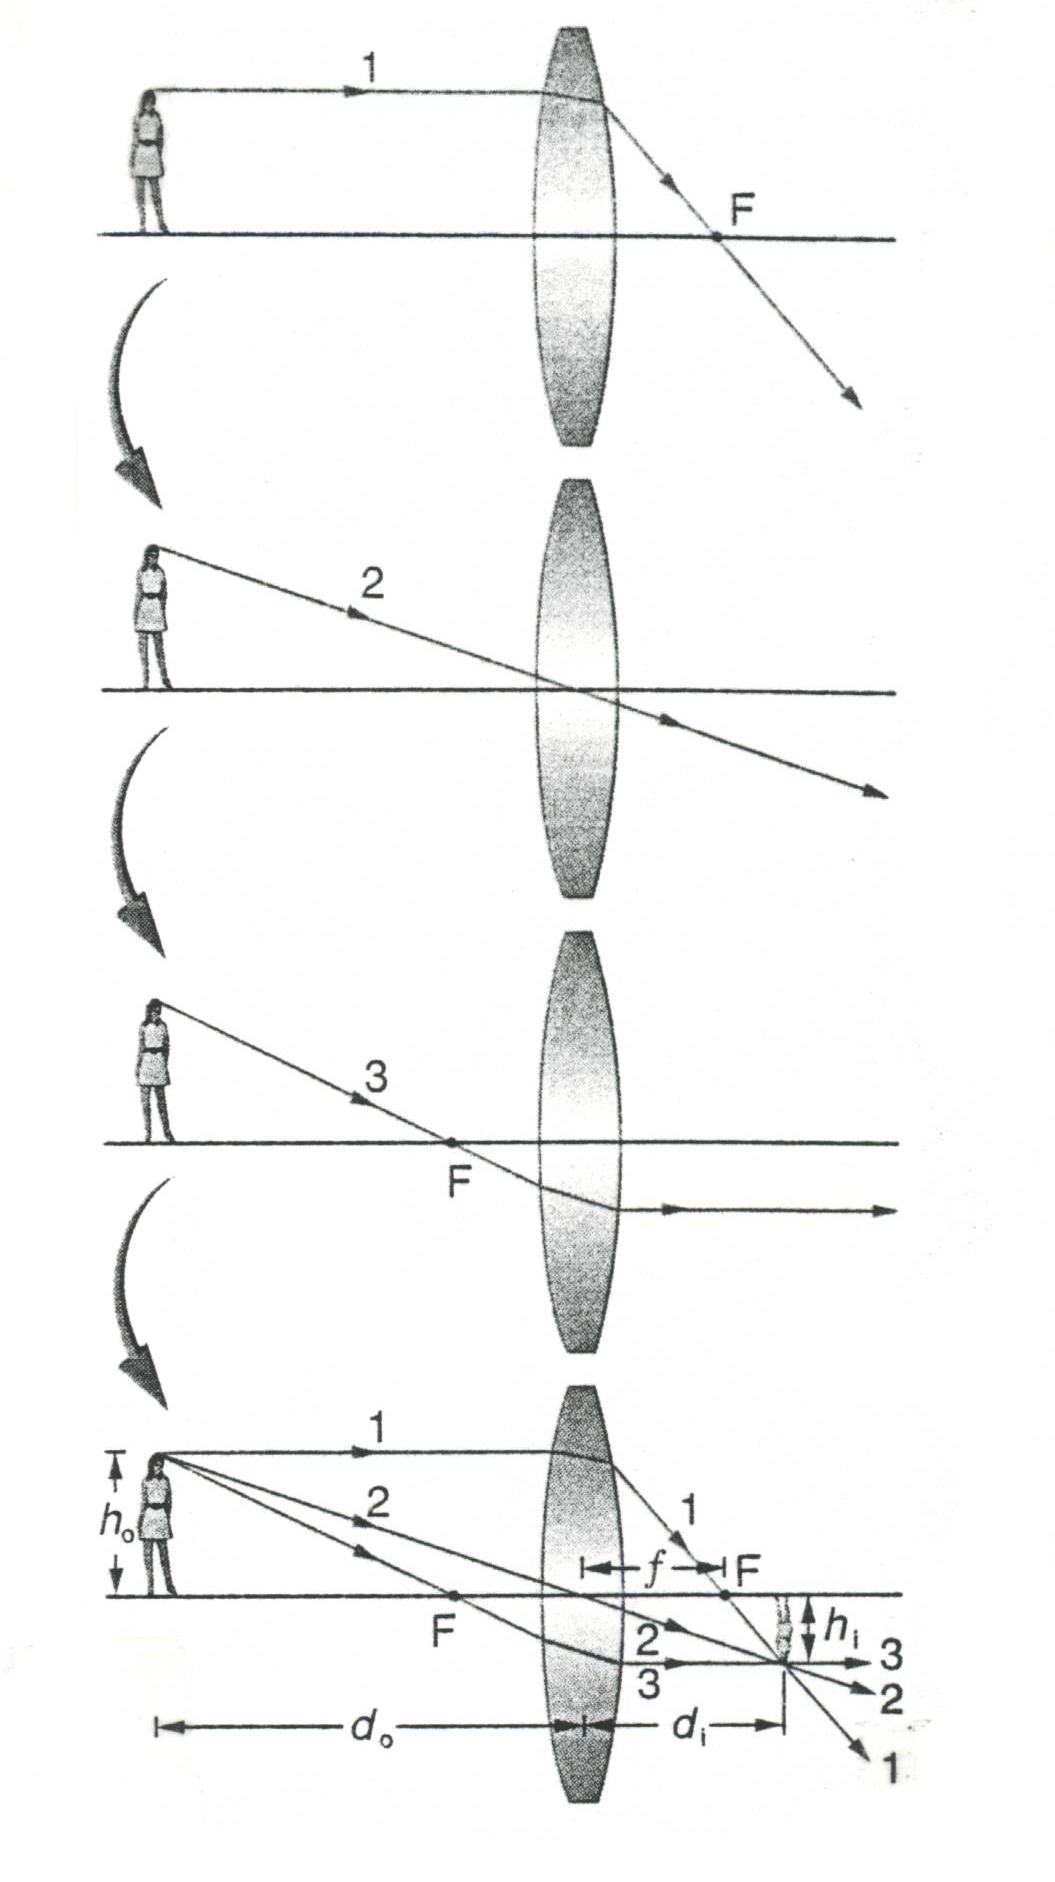
\includegraphics[scale=0.7]{5bgraf/fig_17}
	\mfcaption{Ray tracing is used to locate the image formed by a lens}
	\label{f:fig17}
\end{center}

The thin lens equations give the relationships of various quantities involved with thin lenses.  Note that the thin lens calculations produce results consistent with ray tracing and are in fact a numerical equivalent to the graphical techniques of ray tracing.

The object, $d_o$ and image, $d_i$ distances are related to the lens focal length $f$ by the thin lens equation, while the magnification is related to the distances, and to the image and object heights.

\begin{equation} \label{e:thin}
	\frac{1}{d_o} + \frac{1}{d_i} = \frac{1}{f}
\end{equation}
and
\begin{equation} \label{e:thinmag}
	\frac{h_i}{h_o} = -\frac{d_i}{d_o} = m
\end{equation}

\paragraph{Note} Your textbook may use different names for object and image distances, such as $p$ and $q$, or $s$ and $s'$.

%---------------------------------------------------------------------
%\section{Activities}
\section {Thin lenses}
\subsection{Activity: Focal length of a convex lens}\label{s:focal}
\begin{enumerate}[leftmargin=*] 
	\item Determine the focal length $f$ of a convex lens by forming an image of a distant object.  The object should be something you can see out the lab window.
	\item Explain your technique and estimate the uncertainty in your value for $f$
\end{enumerate}

\subsection{Activity: Images formed by a single thin lens}\label{s:thinlens}
\begin{enumerate}[leftmargin=*] 
	\item Using the optical bench, the light source, and the hooded screen, find the image location experimentally for the six situations below. For the first five, use the converging lens whose focal length $f$ you measured in activity \ref{s:focal}. Make a table in which you list values and uncertainties for the measured quantities $d_o$ (cm), $d_i$ (cm), $h_o$ (cm), $h_i$ (cm), and  $m$ for each of the five situations.
	\item Make room in your table for two other columns -- one for the calculated value of $d_i$ (cm) and another for the calculated value of $m$.
\end{enumerate}
	
\hrule	
\begin{equation*}
\begin{array}{llll}
	\text{(i)}	& d_o > 2f		& \text{(ii)}	& d_o = 2f \\
	\text{(iii)}	& f < d_o < 2f	& \text{(iv)}	& d_o = f \\
	\text{(v)}	& d_o < f 		& \text{(vi)}	& \text{any}\  d_o, \text{negative}\  f
\end{array}
\end{equation*}
		
\subsection{Activity: Image location using thin lens equation}
\begin{enumerate}[leftmargin=*] 
	\item Using the thin lens equation and the measured values of $d_o$ and $f$, calculate the location of the image $d_i$ in each of the first five situations. 
	\item Using the calculated value of $d_i$, find the magnification $m$. Include these calculated values in the table you made above. 
	\item Discuss how well the calculated values match the corresponding measured values. 
	\item In the sixth situation, calculate the focal length of the diverging lens.
	{\item (Measuring the image distance and location is difficult for the sixth situation, and is usually done using the ``parallax'' method, which your instructor will explain to you.)}
\end{enumerate}

\subsection{Activity: Ray tracing}
\begin{enumerate}[leftmargin=*] 
	\item For each of the six situations explored above, draw ray diagrams approximately to scale. Use graph paper, ruler, and thin lines to get the best results. Discuss any trends you observe. 
	\item Note the correspondence between the ray diagrams and the quantities measured in activity \ref{s:thinlens}.
\end{enumerate}

%---------------------------------------------------------------------
\section{Conclusions}
Did you observe the three types of images that can be formed by a single lens? Which of the six situations produced real images? Which produced virtual images? Which produced no image?  

% Questions: State what happens to the image distance as the object distance moves toward the focal point. Assume the object starts at infinity. State what happens to image distance as the object distance moves closer to the lens surface. Assume the object starts at the focal point.

% \clearpage
%\newpage
%\includegraphics*[width=\textwidth,trim=120 80 80 120,clip]{5bgraf/pslabgrid} 
 \end{multicols}
%--------------------------------------------------------------------------
\endinput
%--------------------------------------------------------------------------
